\newpage
\subsubsection{2.4. Kết quả kiểm thử trên mô hình CNN + MGAT + FastKAN/MLP với hai phương thức (hình ảnh và văn bản)}
\indent\indent Dưới đây là kết quả kiểm thử chi tiết của 12 mô hình CNN backbone + MGAT + FastKAN/MLP với hai phương thức (hình ảnh và văn bản), trong đó các giá trị được lấy từ lần chạy đạt kết quả cao nhất.\vspace{0.3cm}

%===================================================================
\textbf{* ResNet18 + MGAT + FastKAN/MLP:} 
\begin{table}[H]
\centering
\renewcommand{\arraystretch}{1.08}
\caption{\centering Classification report của FastKAN(1) và MLP(2) trên hai phương thức với backbone ResNet18}
\begin{tabular}{lccccccc}
\hline \textbf{Lớp} & \textbf{P(1)} & \textbf{R(1)} & \textbf{F1(1)} & \textbf{P(2)} & \textbf{R(2)} & \textbf{F1(2)} & \textbf{Support} \\ \hline

cho-noi-cai-rang
& 0.9130 & 0.9333 & \textbf{0.9231}
& 1.0000 & 0.7556 & 0.8608 & 45 \\

dua-bo-bay-nui
& 0.9783 & 1.0000 & \textbf{0.9890}
& 0.9574 & 1.0000 & 0.9783 & 45 \\

hoi-lim
& 0.9565 & 0.9778 & \textbf{0.9670}
& 0.9773 & 0.9556 & 0.9663 & 45 \\

le-hoi-nghinh-ong
& 0.8286 & 0.6444 & 0.7250
& 0.8333 & 0.7778 & \textbf{0.8046} & 45 \\

nghe-dan-tre
& 0.9783 & 1.0000 & \textbf{0.9890}
& 0.8654 & 1.0000 & 0.9278 & 45 \\

nghe-det-chieu
& 0.9778 & 0.9778 & \textbf{0.9778}
& 0.9512 & 0.8667 & 0.9070 & 45 \\

ok-om-bok
& 1.0000 & 0.9111 & \textbf{0.9535}
& 0.8400 & 0.9333 & 0.8842 & 45 \\

via-ba-chua-xu-nui-sam
& 0.7091 & 0.8667 & \textbf{0.7800}
& 0.8000 & 0.8889 & 0.8421 & 45 \\
\hline

\textbf{Accuracy}
& & & \textbf{0.9139}
& & & 0.8972 & 360 \\

\textbf{Macro avg}
& \textbf{0.9177} & \textbf{0.9139} & \textbf{0.9130}
& 0.9031 & 0.8972 & 0.8964 & 360 \\

\textbf{Weighted avg}
& \textbf{0.9177} & \textbf{0.9139} & \textbf{0.9130}
& 0.9031 & 0.8972 & 0.8964 & 360 \\
\hline
\end{tabular}
\end{table}

%===================================================================
\textbf{* RegNetX400MF + MGAT + FastKAN/MLP:}
\begin{table}[H]
\centering
\renewcommand{\arraystretch}{1.08}
\caption{\centering Classification report của FastKAN(1) và MLP(2) trên hai phương thức với backbone RegNetX400MF}
\begin{tabular}{lccccccc}
\hline \textbf{Lớp} & \textbf{P(1)} & \textbf{R(1)} & \textbf{F1(1)} & \textbf{P(2)} & \textbf{R(2)} & \textbf{F1(2)} & \textbf{Support} \\ \hline

cho-noi-cai-rang
& 0.8600 & 0.9556 & 0.9053 
& 0.9149 & 0.9556 & \textbf{0.9348} & 45 \\

dua-bo-bay-nui 
& 0.9574 & 1.0000 & 0.9783 
& 0.9783 & 1.0000 & \textbf{0.9890} & 45 \\

hoi-lim 
& 0.8113 & 0.9556 & 0.8776 
& 0.9333 & 0.9333 & \textbf{0.9333} & 45 \\

le-hoi-nghinh-ong
& 0.7234 & 0.7556 & 0.7391 
& 0.7500 & 0.8000 & \textbf{0.7742} & 45 \\

nghe-dan-tre
& 1.0000 & 0.9778 & 0.9888 
& 0.9783 & 1.0000 & \textbf{0.9890} & 45 \\

nghe-det-chieu 
& 0.9487 & 0.8222 & 0.8810 
& 0.9556 & 0.9556 & \textbf{0.9556} & 45 \\

ok-om-bok 
& 0.9737 & 0.8222 & 0.8916 
& 0.9545 & 0.9333 & \textbf{0.9438} & 45 \\

via-ba-chua-xu-nui-sam 
& 0.7381 & 0.6889 & 0.7126 
& 0.8718 & 0.7556 & \textbf{0.8095} & 45 \\
\hline

\textbf{Accuracy}
& & & 0.8722
& & & \textbf{0.9167}  & 360 \\

\textbf{Macro avg} 
& 0.8766 & 0.8722 & 0.8718 
& \textbf{0.9171} & \textbf{0.9167} & \textbf{0.9162} & 360 \\

\textbf{Weighted avg}
& 0.8766 & 0.8722 & 0.8718 
& \textbf{0.9171} & \textbf{0.9167} & \textbf{0.9162} & 360 \\
\hline
\end{tabular}
\end{table}
%===================================================================
\newpage
\textbf{* MobileNetV3 Large + MGAT + FastKAN/MLP:}
\begin{table}[H]
\centering
\renewcommand{\arraystretch}{1.08}
\caption{\centering Classification report của FastKAN(1) và MLP(2) trên hai phương thức với backbone MobileNetV3 Large}
\begin{tabular}{lccccccc}
\hline \textbf{Lớp} & \textbf{P(1)} & \textbf{R(1)} & \textbf{F1(1)} & \textbf{P(2)} & \textbf{R(2)} & \textbf{F1(2)} & \textbf{Support} \\ \hline

cho-noi-cai-rang 
& 0.8824 & 1.0000 & \textbf{0.9375} 
& 0.9149 & 0.9556 & 0.9348 & 45 \\

dua-bo-bay-nui
& 1.0000 & 1.0000 & \textbf{1.0000}
& 1.0000 & 1.0000 & \textbf{1.0000} & 45 \\

hoi-lim 
& 0.9333 & 0.9333 & \textbf{0.9333} 
& 0.8182 & 1.0000 & 0.9000 & 45 \\

le-hoi-nghinh-ong
& 0.9032 & 0.6222 & 0.7368 
& 0.9118 & 0.6889 & \textbf{0.7848} & 45 \\

nghe-dan-tre 
& 0.9783 & 1.0000 & \textbf{0.9890} 
& 0.9783 & 1.0000 & \textbf{0.9890} & 45 \\

nghe-det-chieu 
& 1.0000 & 0.9556 & \textbf{0.9773} 
& 0.9762 & 0.9111 & 0.9425 & 45 \\

ok-om-bok 
& 0.9778 & 0.9778 & \textbf{0.9778} 
& 0.9778 & 0.9778 & \textbf{0.9778} & 45 \\

via-ba-chua-xu-nui-sam
& 0.7222 & 0.8667 & 0.7879 
& 0.8043 & 0.8222 & \textbf{0.8132} & 45 \\
\hline

\textbf{Accuracy}
& & & \textbf{0.9194}
& & & \textbf{0.9194} & 360 \\

\textbf{Macro avg} 
& \textbf{0.9246} & \textbf{0.9194} & 0.9175 
& 0.9227 & \textbf{0.9194} & \textbf{0.9178} & 360 \\

\textbf{Weighted avg} 
& \textbf{0.9246} & \textbf{0.9194} & 0.9175 
& 0.9227 & \textbf{0.9194} & \textbf{0.9178} & 360 \\
\hline
\end{tabular}
\end{table}
%===================================================================
\textbf{* MobileNetV3 Small + MGAT + FastKAN/MLP:}
\begin{table}[H]
\centering
\renewcommand{\arraystretch}{1.08}
\caption{\centering Classification report của FastKAN(1) và MLP(2) trên hai phương thức với backbone MobileNetV3 Small}
\begin{tabular}{lccccccc}
\hline \textbf{Lớp} & \textbf{P(1)} & \textbf{R(1)} & \textbf{F1(1)} & \textbf{P(2)} & \textbf{R(2)} & \textbf{F1(2)} & \textbf{Support} \\ \hline

cho-noi-cai-rang 
& 0.7627 & 1.0000 & 0.8654 
& 0.8980 & 0.9778 & \textbf{0.9362} & 45 \\

dua-bo-bay-nui
& 1.0000 & 0.9556 & \textbf{0.9773} 
& 1.0000 & 0.9556 & \textbf{0.9773} & 45 \\

hoi-lim
& 0.9070 & 0.8667 & 0.8864 
& 0.8936 & 0.9333 & \textbf{0.9130} & 45 \\

le-hoi-nghinh-ong
& 0.7879 & 0.5778 & \textbf{0.6667} 
& 0.7027 & 0.5778 & 0.6341 & 45 \\

nghe-dan-tre
& 0.9574 & 1.0000 & \textbf{0.9783} 
& 1.0000 & 0.9333 & 0.9655 & 45 \\

nghe-det-chieu
& 0.9730 & 0.8000 & 0.8780 
& 0.9333 & 0.9333 & \textbf{0.9333} & 45 \\

ok-om-bok
& 0.9574 & 1.0000 & \textbf{0.9783} 
& 0.9556 & 0.9556 & 0.9556 & 45 \\

via-ba-chua-xu-nui-sam
& 0.6863 & 0.7778 & \textbf{0.7292} 
& 0.6538 & 0.7556 & 0.7010 & 45 \\
\hline

\textbf{Accuracy}
& & & 0.8722
& & & \textbf{0.8778} & 360 \\

\textbf{Macro avg}
& 0.8790 & 0.8722 & 0.8699 
& \textbf{0.8796} & \textbf{0.8778} & \textbf{0.8770} & 360 \\

\textbf{Weighted avg}
& 0.8790 & 0.8722 & 0.8699 
& \textbf{0.8796} & \textbf{0.8778} & \textbf{0.8770} & 360 \\
\hline
\end{tabular}
\end{table}
%===================================================================
\textbf{* DenseNet121 + MGAT + FastKAN/MLP:}
\begin{table}[H]
\centering
\renewcommand{\arraystretch}{1.08}
\caption{\centering Classification report của FastKAN(1) và MLP(2) trên hai phương thức với backbone DenseNet121}
\begin{tabular}{lccccccc}
\hline \textbf{Lớp} & \textbf{P(1)} & \textbf{R(1)} & \textbf{F1(1)} & \textbf{P(2)} & \textbf{R(2)} & \textbf{F1(2)} & \textbf{Support} \\ \hline

cho-noi-cai-ran
& 0.9565 & 0.9778 & \textbf{0.9670} 
& 0.9149 & 0.9556 & 0.9348 & 45 \\

dua-bo-bay-nui 
& 0.9375 & 1.0000 & 0.9677 
& 1.0000 & 1.0000 & \textbf{1.0000} & 45 \\

hoi-lim 
& 0.8980 & 0.9778 & \textbf{0.9362} 
& 0.9756 & 0.8889 & 0.9302 & 45 \\

le-hoi-nghinh-ong
& 0.7692 & 0.8889 & 0.8247 
& 0.7843 & 0.8889 & \textbf{0.8333} & 45 \\

nghe-dan-tre
& 0.9783 & 1.0000 & \textbf{0.9890} 
& 1.0000 & 0.9333 & 0.9655 & 45 \\

nghe-det-chieu 
& 1.0000 & 0.9333 & \textbf{0.9655} 
& 0.9111 & 0.9111 & 0.9111 & 45 \\

ok-om-bok
& 0.9744 & 0.8444 & 0.9048 
& 0.9149 & 0.9556 & \textbf{0.9348} & 45 \\

via-ba-chua-xu-nui-sam
& 0.8421 & 0.7111 & 0.7711 
& 0.8571 & 0.8000 & \textbf{0.8276} & 45 \\
\hline

\textbf{Accuracy}
& & & \textbf{0.9167}
& & & \textbf{0.9167} & 360 \\

\textbf{Macro avg} 
& 0.9195 & 0.9167 & 0.9158 
& \textbf{0.9197} & \textbf{0.9167} & \textbf{0.9172} & 360 \\

\textbf{Weighted avg}
& 0.9195 & 0.9167 & 0.9158 
& \textbf{0.9197} & \textbf{0.9167} & \textbf{0.9172} & 360 \\
\hline
\end{tabular}
\end{table}

%===================================================================
\textbf{* ShuffleNetV2 1.0x + MGAT + FastKAN/MLP:}
\begin{table}[H]
\centering
\renewcommand{\arraystretch}{1.08}
\caption{\centering Classification report của FastKAN(1) và MLP(2) trên hai phương thức với backbone ShuffleNetV2 1.0x}
\begin{tabular}{lccccccc}
\hline \textbf{Lớp} & \textbf{P(1)} & \textbf{R(1)} & \textbf{F1(1)} & \textbf{P(2)} & \textbf{R(2)} & \textbf{F1(2)} & \textbf{Support} \\ \hline

cho-noi-cai-rang
& 0.9545 & 0.9333 & \textbf{0.9438}
& 0.9535 & 0.9111 & 0.9318 & 45 \\

dua-bo-bay-nui
& 0.8958 & 0.9556 & 0.9247
& 0.9149 & 0.9556 & \textbf{0.9348} & 45 \\

hoi-lim
& 0.9167 & 0.9778 & \textbf{0.9462}
& 0.8980 & 0.9778 & 0.9362 & 45 \\

le-hoi-nghinh-ong
& 0.8085 & 0.8444 & 0.8261
& 0.8780 & 0.8000 & \textbf{0.8372} & 45 \\

nghe-dan-tre
& 0.9184 & 1.0000 & \textbf{0.9574}
& 0.9767 & 0.9333 & 0.9545 & 45 \\

nghe-det-chieu
& 0.9756 & 0.8889 & \textbf{0.9302}
& 0.8958 & 0.9556 & 0.9247 & 45 \\

ok-om-bok
& 0.9268 & 0.8444 & 0.8837
& 0.9737 & 0.8222 & \textbf{0.8916} & 45 \\

via-ba-chua-xu-nui-sam
& 0.8571 & 0.8000 & \textbf{0.8276}
& 0.7647 & 0.8667 & 0.8125 & 45 \\
\hline

\textbf{Accuracy}
& & & \textbf{0.9056}
& & & 0.9028 & 360 \\

\textbf{Macro avg}
& 0.9067 & \textbf{0.9056} & \textbf{0.9050}
& \textbf{0.9069} & 0.9028 & 0.9029 & 360 \\

\textbf{Weighted avg}
& 0.9067 & \textbf{0.9056} & \textbf{0.9050}
& \textbf{0.9069} & 0.9028 & 0.9029 & 360 \\
\hline
\end{tabular}
\end{table}

\indent Dựa trên kết quả kiểm thử với các mô hình trên hai phương thức (hình ảnh và văn bản), tôi rút ra các nhận xét sau: \vspace{-0.1cm}
\begin{itemize}[label={--}, itemsep=1pt]
    \item \textbf{Sự cải thiện vượt bậc ở các mô hình nhẹ:} 
    Trái ngược với các mô hình lớn, các kiến trúc nhẹ lại hưởng lợi nhiều nhất từ việc bổ sung dữ liệu văn bản. Điển hình là ShuffleNetV2 1.0x, từ mức thấp nhất ở baseline (0.8222), khi kết hợp MGAT + FastKAN thì kết quả lại đạt tới 0.9056, kết hợp với MLP cũng rất tốt với kết quả đạt 0.9028 (tăng gần 8\%). Tương tự, MobileNetV3 Small cũng ghi nhận mức tăng đáng kể khoảng 2.2\% (từ 0.8472 lên 0.8778). Điều này chứng minh kiến trúc đồ thị đa phương thức mang lại hiệu quả trong việc bù đắp sự thiếu hụt thông tin của các backbone nhỏ.

    \item \textbf{Vấn đề với RegNetX400MF:}
    Trong khi hầu hết các mô hình đều tăng hoặc giữ ổn định, RegNetX400MF kết hợp FastKAN lại cho thấy sự sụt giảm độ chính xác so với baseline (0.8722 so với 0.8806). Tuy nhiên, khi chuyển sang dùng bộ phân lớp MLP, kết quả lại thiên về mức tốt hơn (0.9167). Điều này cho thấy đặc trưng của RegNet có thể không tương thích tốt với cấu trúc lưới của FastKAN trong không gian đa phương thức này.

    \item \textbf{Chưa cải thiện mạnh trên một số mô hình:} 
    Với các kiến trúc mạnh như DenseNet121, ResNet18, và MobileNet V3 Large sự cải thiện là có nhưng không quá đột biến (tăng nhẹ khoảng 0.3\% -- 1\% so với baseline). Điều này dễ hiểu vì bản thân các mô hình này đã khai thác rất tốt thông tin hình ảnh, nên phần thông tin bổ trợ từ văn bản chỉ đóng vai trò tinh chỉnh nhỏ ở các biên quyết định khó.
\end{itemize}

%===================================================================
\begin{table}[H]
\centering
\renewcommand{\arraystretch}{1.2}
\setlength{\tabcolsep}{6pt}
\caption{\centering Kết quả kiểm thử trung bình của tất cả các mô hình CNN backbone + MGAT + FastKAN/MLP trên hai phương thức}
\begin{tabular}{llcccc}
\hline
\textbf{Backbone Model (+ MGAT)} & \textbf{Classifier} & \textbf{Accuracy} & \textbf{Precision} & \textbf{Recall} & \textbf{F1-Score} \\
\hline

% ResNet18
\multirow{2}{*}{ResNet18} 
& FastKAN & \textbf{0.8962} & \textbf{0.8993} & \textbf{0.8963} & \textbf{0.8958} \\
& MLP & 0.8843 & 0.8889 & 0.8843 & 0.8834 \\
\hline

% RegNetX400MF
\multirow{2}{*}{RegNetX400MF} 
& FastKAN & 0.8648 & 0.8814 & 0.8648 & 0.8643 \\
& MLP & \textbf{0.8926} & \textbf{0.8942} & \textbf{0.8926}
& \textbf{0.8921} \\
\hline

% MobileNetV3 Large
\multirow{2}{*}{MobileNetV3 Large} 
& FastKAN & 0.9111 & 0.9143 & 0.9111 & 0.9098 \\
& MLP & \textbf{0.9157} & \textbf{0.9177} & \textbf{0.9157} & \textbf{0.9147} \\
\hline

% MobileNetV3 Small
\multirow{2}{*}{MobileNetV3 Small} 
& FastKAN & 0.8583 & 0.8615 & 0.8583 & 0.8557 \\
& MLP & \textbf{0.8694} & \textbf{0.8726} & \textbf{0.8694} & \textbf{0.8687} \\
\hline

% DenseNet121
\multirow{2}{*}{DenseNet121} 
& FastKAN & \textbf{0.9083} & \textbf{0.9102} & \textbf{0.9083} & \textbf{0.9082} \\
& MLP & 0.9037 & 0.9066 & 0.9037 & 0.9028 \\
\hline

% ShuffleNetV2
\multirow{2}{*}{ShuffleNetV2 1.0x} 
& FastKAN & \textbf{0.8982} & 0.8988 & \textbf{0.8982} & \textbf{0.8973} \\
& MLP & 0.8917 & \textbf{0.8989} & 0.8917 & 0.8916 \\
\hline

\end{tabular}
\label{tab:avg_performance_comparison_v2}
\end{table}

\begin{figure}[H]
    \centering
    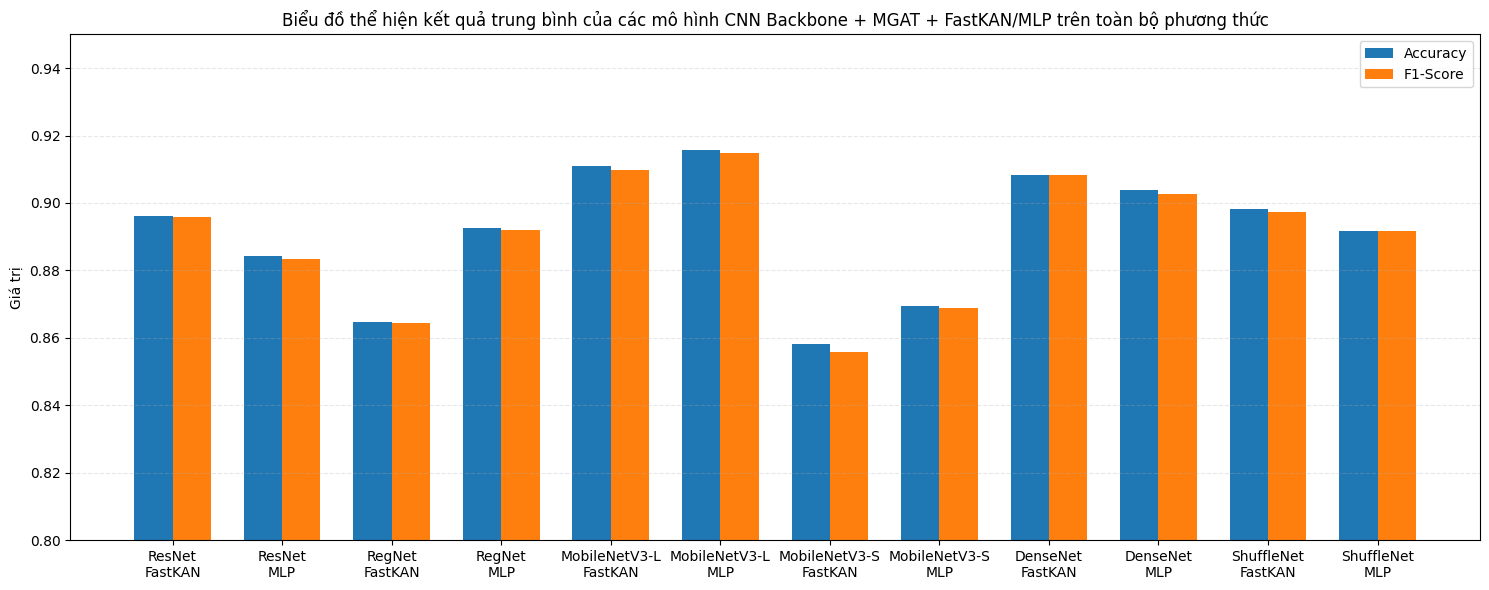
\includegraphics[width=\linewidth]{images/part-02/chap-03/sec-02/PipelineImageText.png}
    \caption{\centering Biểu đồ thể hiện kết quả kiểm thử trung bình của tất cả các mô hình CNN backbone + MGAT + FastKAN/MLP trên hai phương thức}
    \label{fig:KQPipelineImageText}
\end{figure}

\indent Dựa trên bảng tổng hợp và biểu đồ thể hiện kết quả trung bình của 12 mô hình trên hai phương thức, tôi đưa ra các kết luận sau:\vspace{-0.1cm}
\begin{itemize}[label={--}, itemsep=1pt]
    \item \textbf{Sự hụt hơi của FastKAN:} So với sự cải thiện vượt trội trên ba phương thức (ví dụ: ResNet18 tăng hơn 3\% so với MLP), thì ở kịch bản hai phương thức, sự cải thiện của FastKAN là không đáng kể (cao hơn \textasciitilde 1\%). Điều này cho thấy rằng FastKAN cần thêm nguồn thông tin đầu vào phong phú và đa dạng hơn để phát huy tối đa ưu thế về khả năng xấp xỉ hàm phi tuyến. Khi không gian đặc trưng đầu vào bị thu hẹp (do thiếu dữ liệu âm thanh), các mối quan hệ ngữ nghĩa trở nên đơn giản hơn, khiến cho kiến trúc phức tạp của KAN chưa được tận dụng triệt để, dẫn đến khoảng cách hiệu năng bị thu hẹp lại so với mạng MLP truyền thống.

    \item \textbf{Sự ổn định của MLP trên MobileNet và RegNet:} 
    Ngược lại, với dòng MobileNetV3 và RegNetX400MF, MLP luôn cho kết quả nhỉnh hơn hoặc ổn định hơn FastKAN. Điển hình là trường hợp RegNetX400MF, MLP đạt độ chính xác 0.8926, bỏ xa mức 0.8648 của FastKAN. Điều này cho thấy đối với dạng đặc trưng được trích xuất từ các backbone này, cấu trúc tuyến tính đơn giản của MLP lại phù hợp và ít rủi ro hơn, tránh được hiện tượng phân tán hoặc khó hội tụ mà FastKAN gặp phải trong trường hợp này.

    \item \textbf{Vai trò thiết yếu của dữ liệu âm thanh:} Dù mô hình hai phương thức đã cho thấy sự cải thiện so với CNN Baseline, nhưng khi đối chiếu với kết quả 3 phương thức (Mục 2.3), ta vẫn nhận thấy sự chênh lệch rõ rệt về độ chính xác (thấp hơn khoảng 2-3\%). Khoảng cách này là minh chứng thực nghiệm cho thấy đối với các di sản văn hóa dạng diễn xướng hoặc lễ hội, thông tin từ kênh âm thanh là mảnh ghép không thể thiếu để hệ thống đạt được hiệu năng tốt hơn.
\end{itemize}